	\documentclass[slidestop,uncompress,mathsans, 12pt]{beamer}
\usepackage[OT1]{eulervm}
%\usepackage[bars]{beamerthemetree}
\usepackage{xcolor}
\usepackage{graphicx}
\usepackage{array}
\usepackage{subfigure}
\usepackage[display]{texpower}
\usepackage{color}
%\usepackage{mathrsfs}
\usetheme{Frankfurt}
\setbeamercolor{alerted text}{fg=red}
%\beamertemplateshadingbackground{blue!5}{yellow!10}
\usecolortheme{whale}
\beamertemplateballitem
%\transglitter[direction=315]

%\useoutertheme{infolines}
%\title[Runzi Qin \space \space \space Rui Guo \space \space \space Yumeng He]{Qin Runzi}
%\subtitle{dsf}
%\institute{Shandong University}
%\date[march 10]{\today}
%\author[Runzi Qin]
\begin{document}
\begin{frame}
\title{The Fall of Hong Kong's Economy}
\subtitle{-----The Analysis of Reasons Behind}
\author{Runzi Qin\\   Hongmei Huang\\   Wanyun Hu\\ Jianing Zhang}
\institute{Shandong University}
\titlepage
\end{frame}

\section{Roadmap}
\subsection{Roadmap}
\begin{frame}
\frametitle{Roadmap}
\begin{itemize}
\item Introduction
\item Internal cause
\item External cause
\begin{enumerate}
\item  Return of Hong Kong
\item  Economic crisis
\item  The rise of mainland China
\end{enumerate}

\item  Conclusion
\end{itemize}
\end{frame}
\section{Introduction}
\subsection{intro}
\begin{frame}{Introduction}
Became a colony $\Longrightarrow$
 Mainly transit trade $\Longrightarrow$
 Industrial city $\Longrightarrow$
 Diversification\\
\bigskip
\begin{figure}[h]
\centering
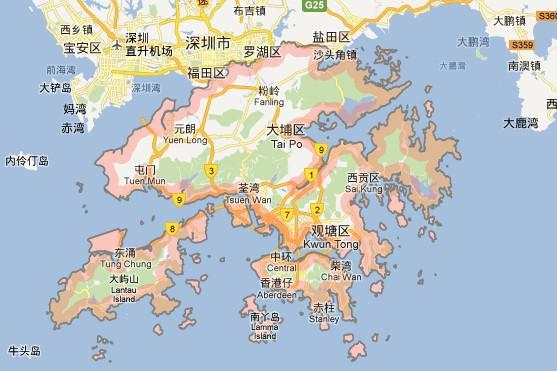
\includegraphics[width=0.6\textwidth]{hk16.jpg}
\label{threadsVsSync}
\caption{Hong Kong map}
\end{figure}
\end{frame}
\section{Internal causes}
\subsection{competitive}
\begin{frame}

\title{The Economic Competitiveness of Hong Kong}
\date{}
\titlepage
\end{frame}
\begin{frame}
\frametitle{The Economic Competitiveness of Hong Kong}
\textcolor{red}{a. The competitiveness analysis of Hong Kong}\\
\begin{overprint}
\onslide<1>
\begin{figure}[h]
\centering
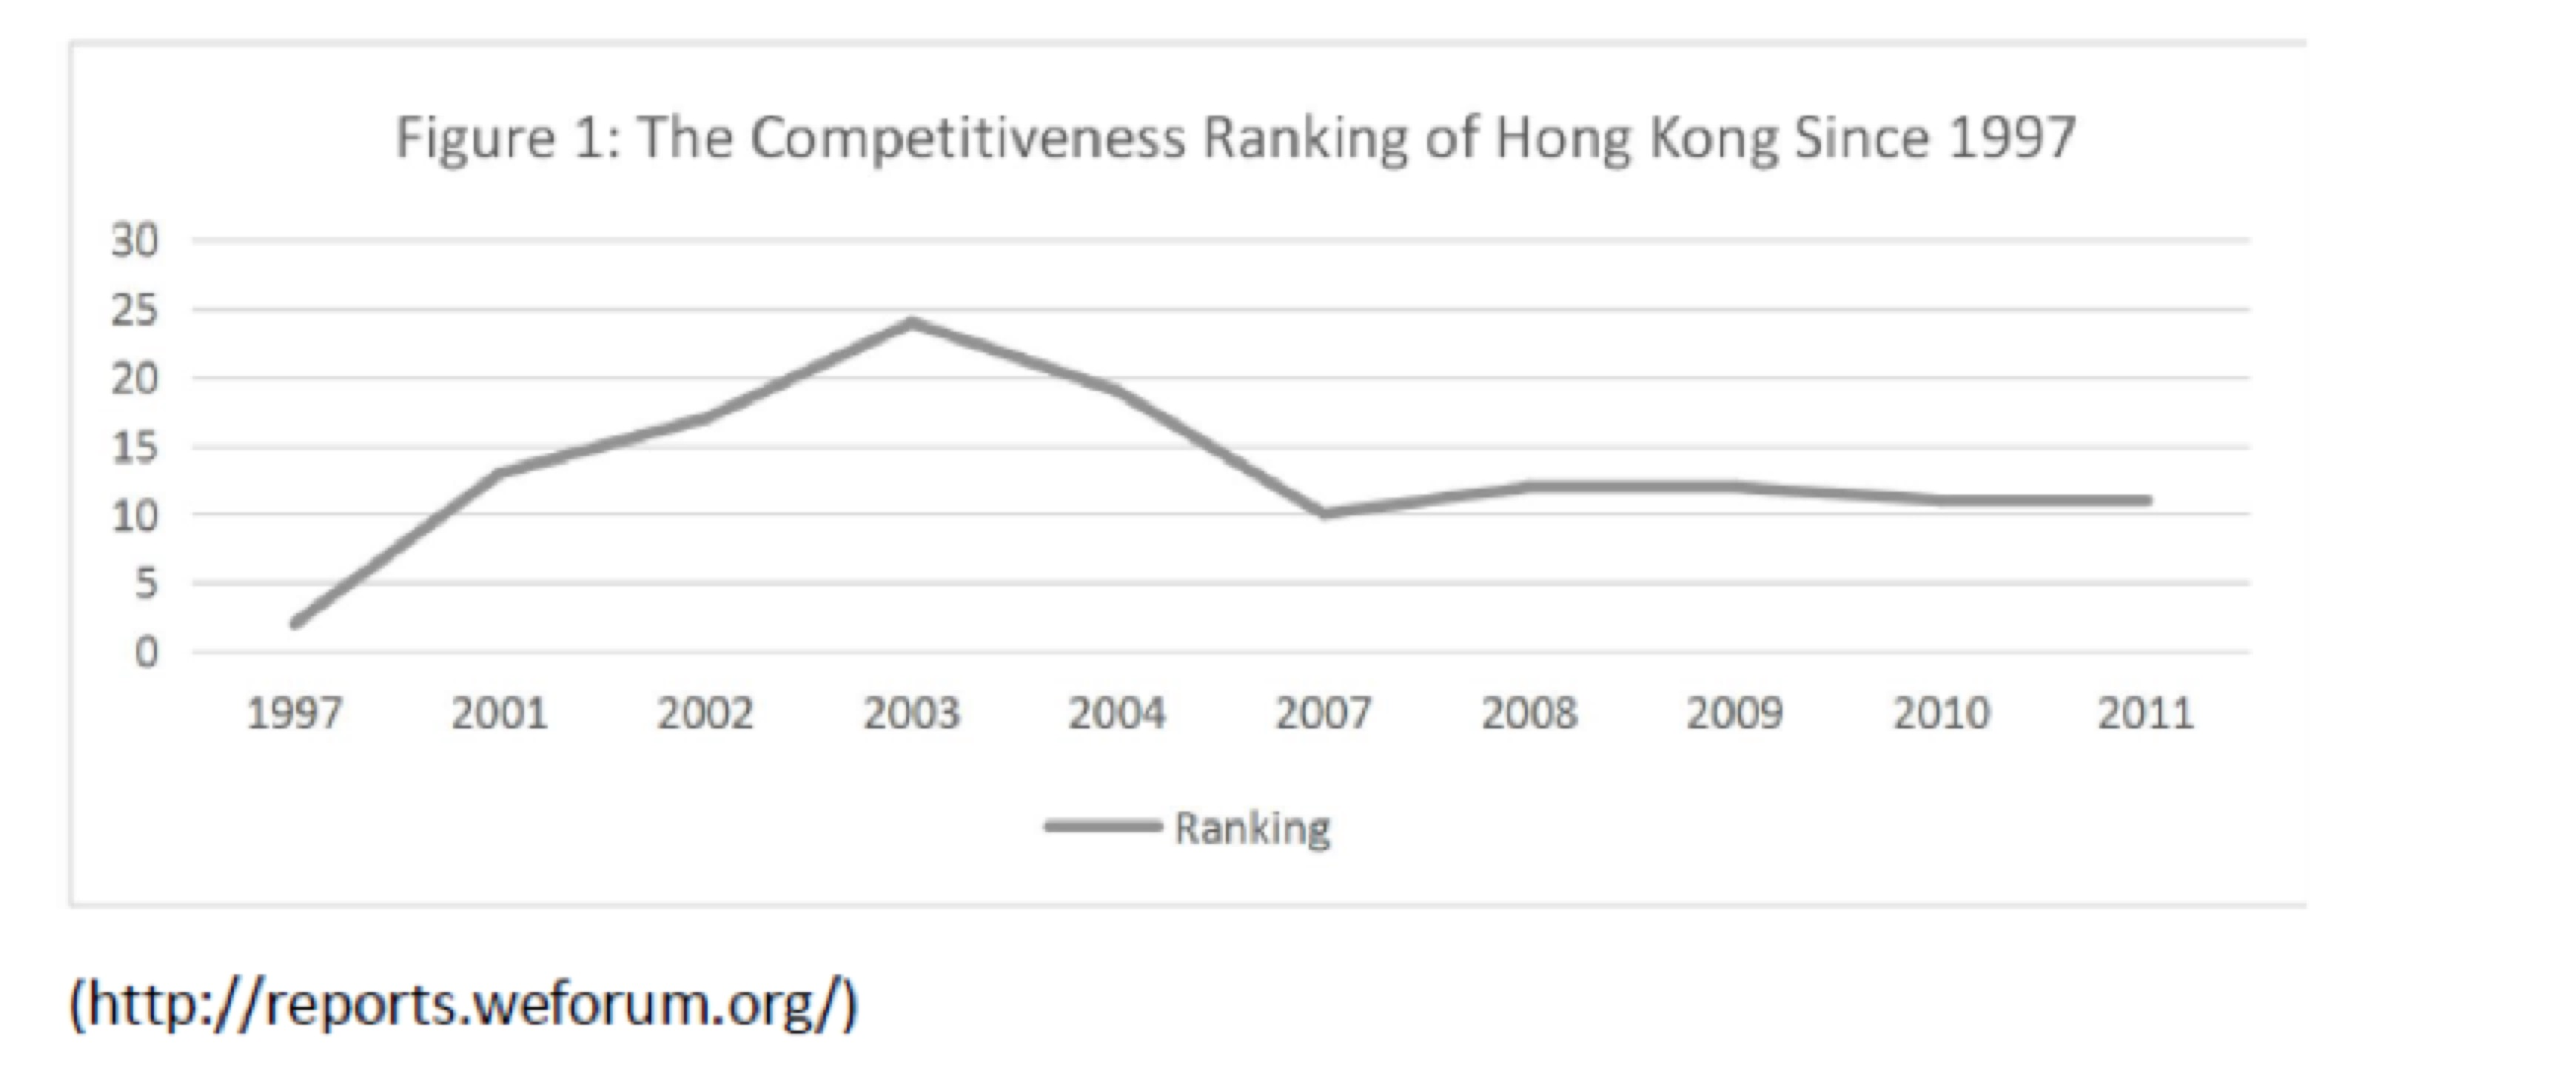
\includegraphics[width=1.1\textwidth]{hk4.jpg}
\label{threadsVsSync}
\end{figure}
\onslide<2>
\begin{figure}[h]
\centering
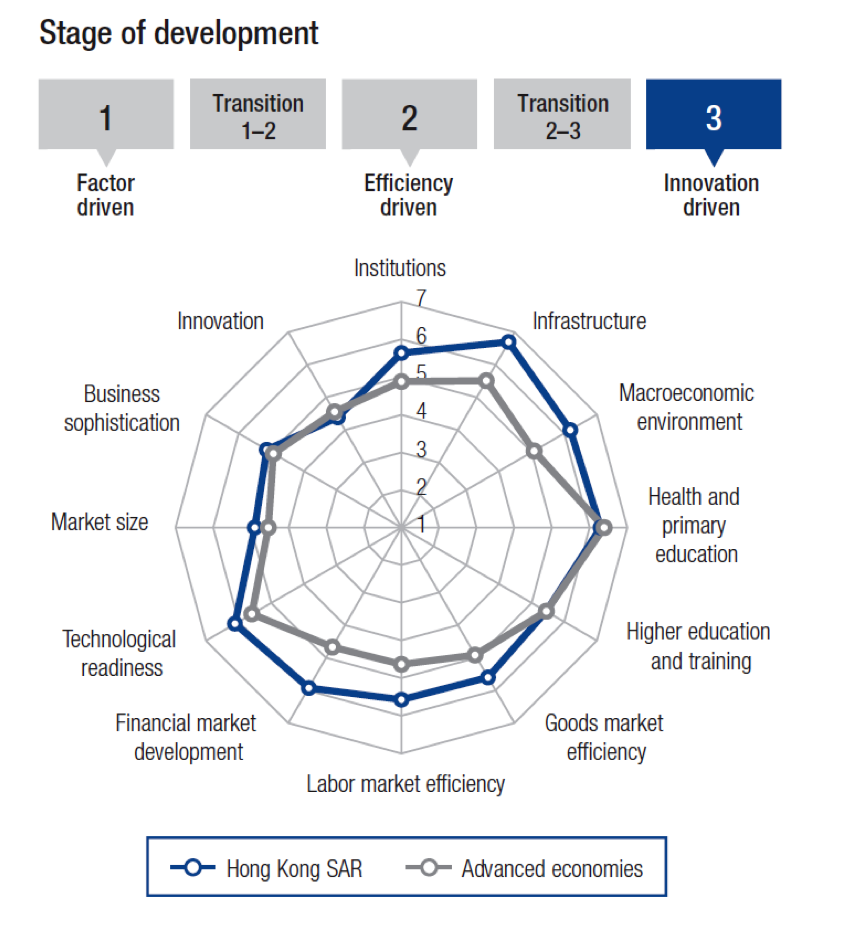
\includegraphics[width=0.5\textwidth]{hk17.png}
\label{threadsVsSync}
\end{figure}
\end{overprint}
\end{frame}

\begin{frame}
\frametitle{The Economic Competitiveness of Hong Kong}%[shrink]
\textcolor{red}{b. The financial market of Hong Kong}\\
And according to Levine (2000) and Arestis (1997), we use the M2/GDP, Loan/M2, Stock market value/GDP to present the competitiveness of Hong Kong financial market.\\
\begin{overprint}
\onslide<1>
\begin{figure}[h]
\centering
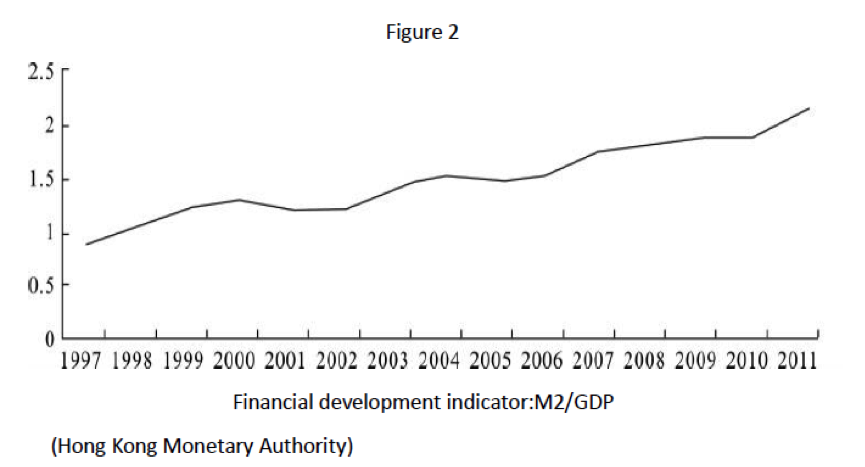
\includegraphics[width=0.8\textwidth]{hk10.png}
\label{threadsVsSync}
\end{figure}
\onslide<2>
\begin{figure}[h]
\centering
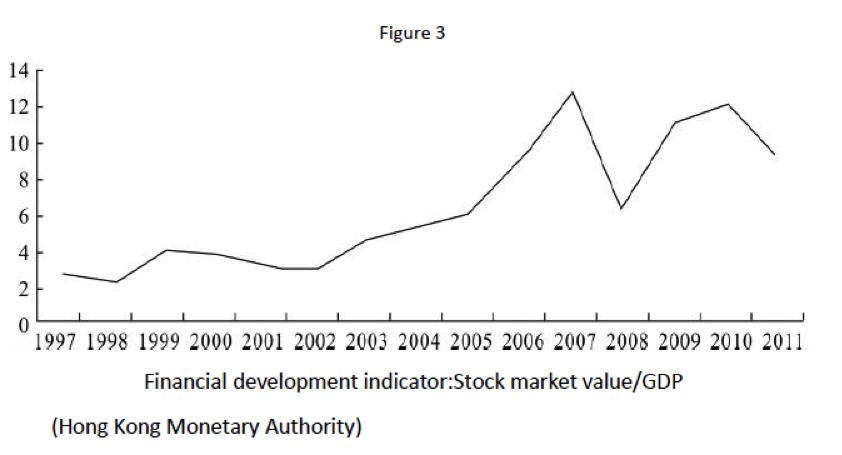
\includegraphics[width=0.8\textwidth]{hk11.png}
\label{threadsVsSync}
\end{figure}
\onslide<3>
\begin{figure}[h]
\centering
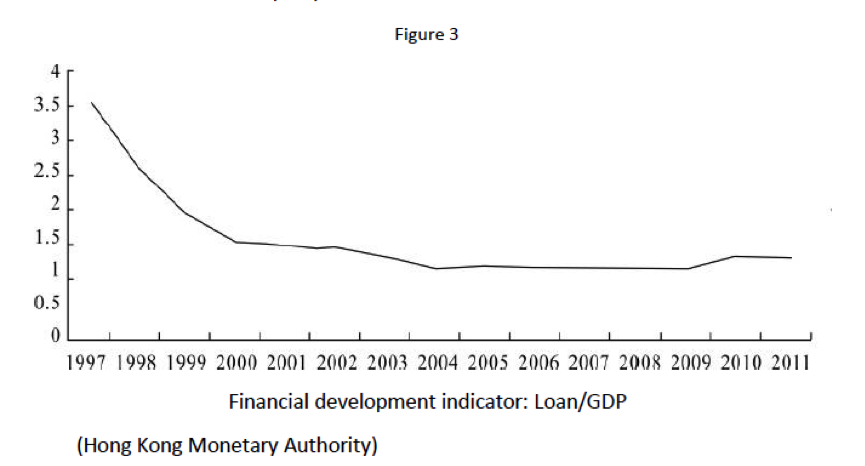
\includegraphics[width=0.8\textwidth]{hk12.png}
\label{threadsVsSync}
\end{figure}
\end{overprint}
\end{frame}
\begin{frame}
\frametitle{The Economic Competitiveness of Hong Kong}
\textcolor{red}{c. The real estate market saturation of Hong Kong}
\begin{overprint}
\onslide<1>
\begin{figure}[h]
\centering
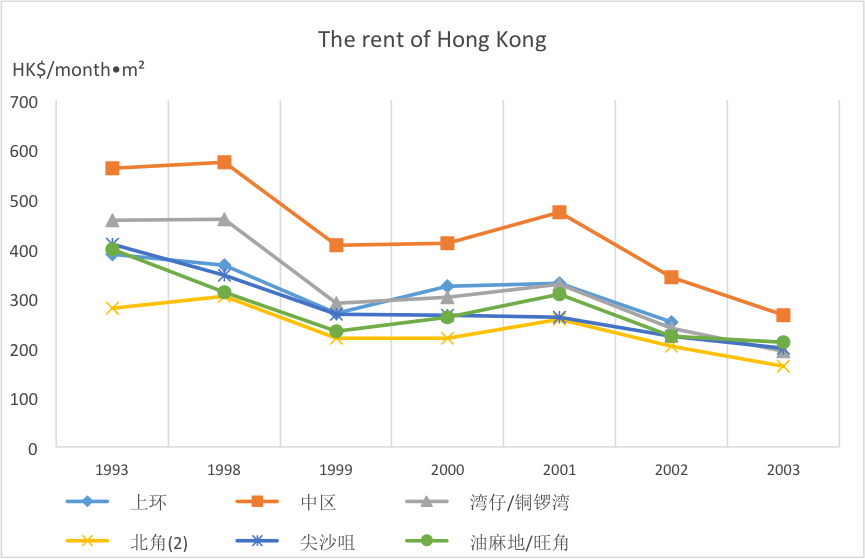
\includegraphics[width=0.8\textwidth]{hk18.png}
\label{threadsVsSync}
\end{figure}
\onslide<2>
\begin{figure}[h]
\centering
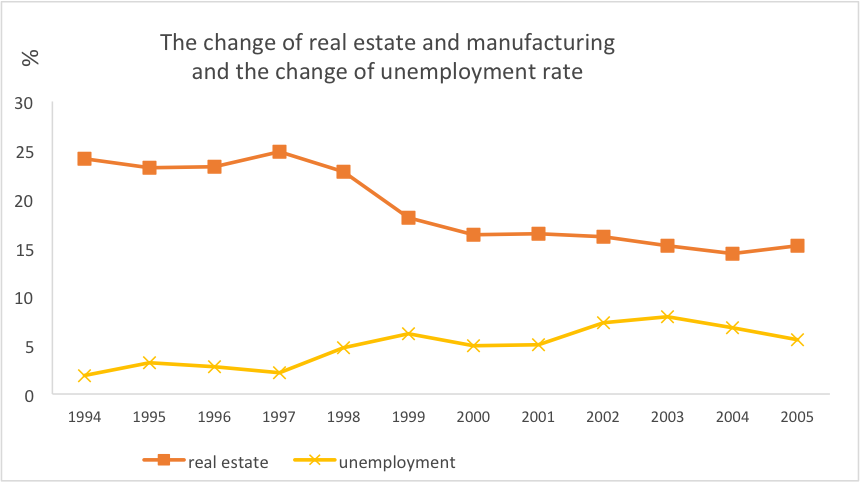
\includegraphics[width=1\textwidth]{hk19.png}
\label{threadsVsSync}
\end{figure}
\onslide<3>
\begin{figure}[h]
\centering
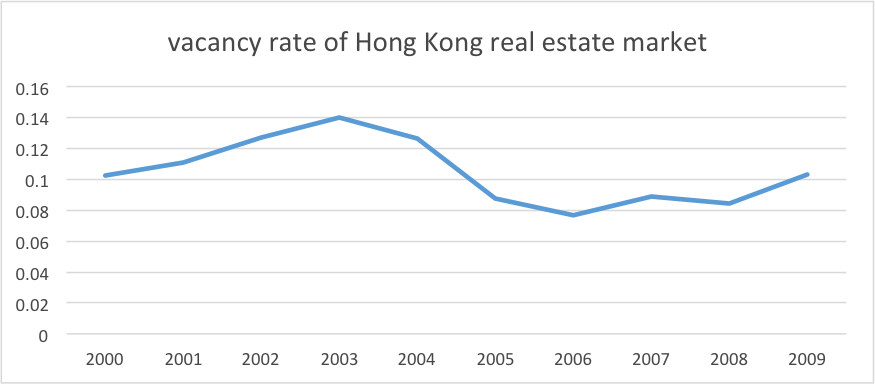
\includegraphics[width=1\textwidth]{hk20.png}
\label{threadsVsSync}
\end{figure}
\end{overprint}
\end{frame}
\begin{frame}{The Economic Competitiveness of Hong Kong}
\textcolor{red}{d. The science and technology competitivness of Hong Kong}\\
\bigskip
Higher education and training ranks 24.
~~Innovation ranks 26 \\
\begin{overprint}
\onslide<1>
\begin{figure}[h]
\centering
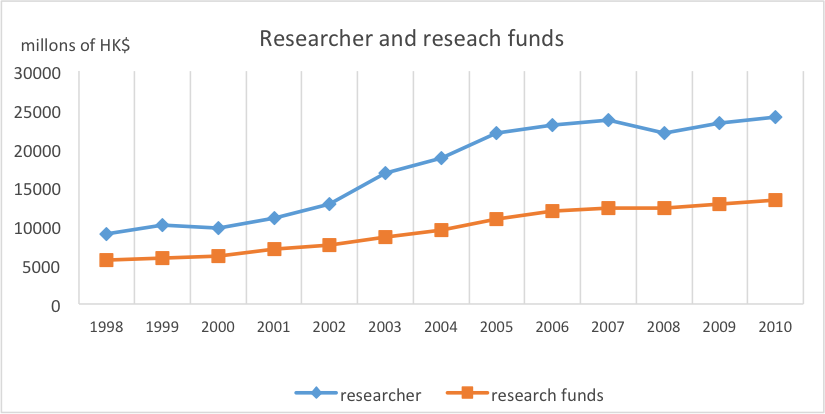
\includegraphics[width=1\textwidth]{hk21.png}
\label{threadsVsSync}
\end{figure}
\onslide<2>
\begin{figure}[h]
\centering
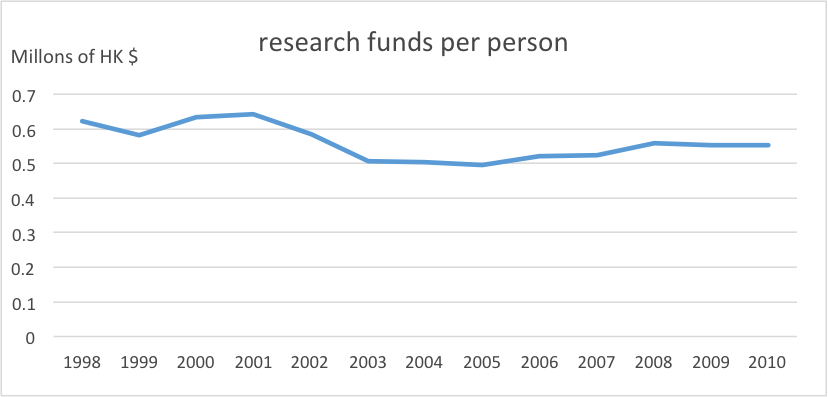
\includegraphics[width=1\textwidth]{hk22.png}
\label{threadsVsSync}
\end{figure}
\end{overprint}
\end{frame}
\section{External causes}
\subsection{azi}
\begin{frame}
\title{Return of Hong Kong}
\date{}
\titlepage
\end{frame}
\begin{frame}
\frametitle{Return of Hong Kong}
\begin{itemize}
\item<2-> \alt<2>{\color{blue} Brain drain and capital flight
}{\color{gray} Brain drain and capital flight
}
\bigskip
\item<2-> \alt<3>{\color{blue} Confliction between Hong Kong and mainland
}{\color{gray} Confliction between Hong Kong and mainland
}
\end{itemize}
\end{frame}
\subsection{sdlkfj}
\begin{frame}
\frametitle{Return of Hong Kong}
Brain Drain and Capital Flight\\
\begin{definition}
\textcolor{cyan}{Brain drain}: a mass emigration of technically skilled people from a country or a region to another country. \\
\bigskip
\textcolor{magenta}{Capital flight}: assets or money rapidly flow out of a country or a region, due to an event of economic consequence. \\

\end{definition}
\end{frame}
\begin{frame}
\begin{figure}[h]
\centering
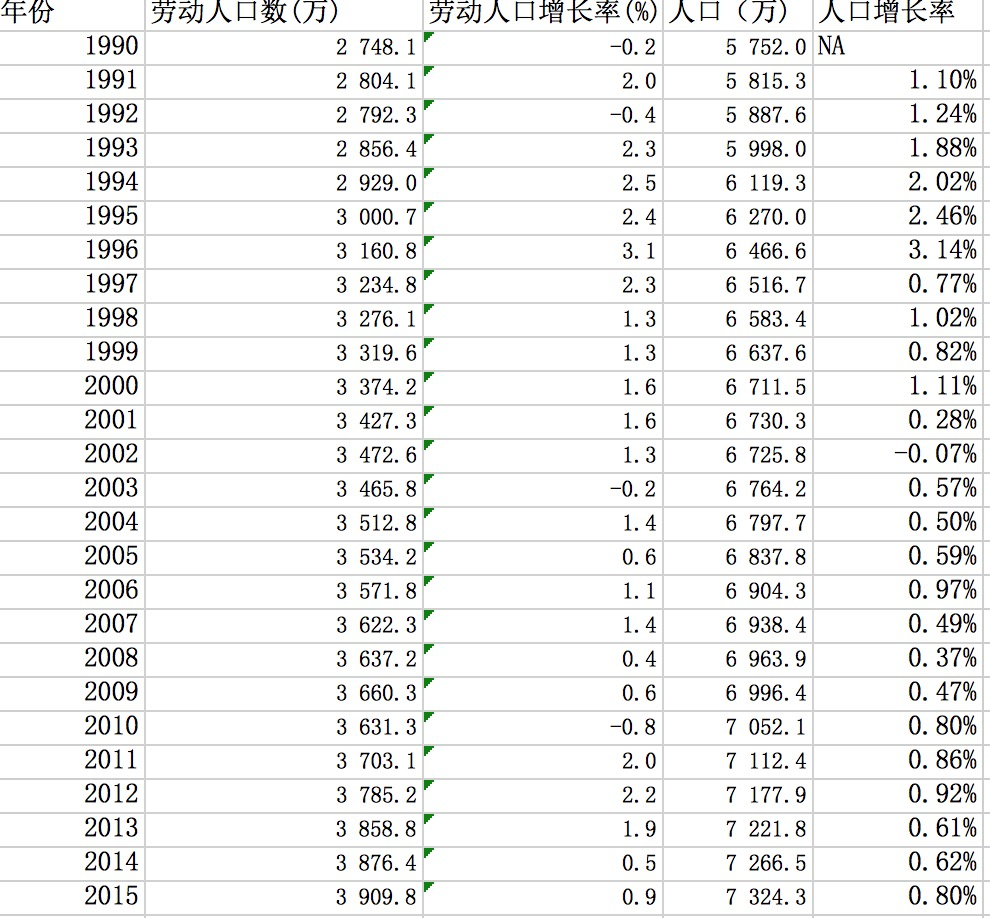
\includegraphics[width=0.8\textwidth]{hk15.jpg}
\label{threadsVsSync}
\end{figure}
\end{frame}
\begin{frame}{Return of Hong Kong}
 Why?
\begin{enumerate}
\item Uncertainty.
\bigskip
\item Better life in other countries.
\end{enumerate}
\end{frame}
\begin{frame}
\frametitle{Return of Hong Kong}
Brain Drain $\Longrightarrow$ Capital Flight
\setbeamercolor{uppercol}{fg=white,bg=blue}%
\setbeamercolor{lowercol}{fg=black,bg=white}%
\begin{beamerboxesrounded}[upper=uppercol,lower=lower col,shadow=true]{Process}
Many capitalists transferred their capital to other countries to avoid the uncertainty of Hong Kong and people who emigrated brought their fortune abroad.\\
\end{beamerboxesrounded}
\end{frame}
\begin{frame}{Return of Hong Kong}
Effect
\begin{block}{}
\center{$Y=A \cdot K^a \cdot L^{1-a}$}
\center{$\Downarrow$\\
\bigskip	Economic Downturn}
\end{block}
\end{frame}
\begin{frame}{Return of Hong Kong}
Confliction between Hong Kong and Mainland\\
\begin{itemize}
\bigskip
\item Institutional difference.
\bigskip
\bigskip
\item Different economic circumstance 
\end{itemize}


\end{frame}
\subsection{Overview}
\begin{frame}
\title{The Influence of Economic Crisis on Hong Kong }
\date{}
\titlepage
\end{frame}
\begin{frame}
\frametitle{The Influence of Economic Crisis on Hong Kong 
}
\begin{itemize}
\item Back ground
\bigskip
\item Data
\bigskip
\item Explanation
\end{itemize}
\end{frame}

\subsection{Background}
\begin{frame}

\frametitle{The Influence of Economic Crisis on Hong Kong }
Background\\
\bigskip
\transglitter[direction=315]
On July 2, 1997, Thailand gave up Fixed Exchange Rates which marked the beginning of Financial Crisis.\\
\end{frame}
\begin{frame}
\frametitle{The Influence of Economic Crisis on Hong Kong }
Background\\
\bigskip
On July 2, 1997, Thailand gave up Fixed Exchange Rates which marked the beginning of Financial Crisis.\\
\bigskip
\transboxin<1>
In 2008, Subprime mortgage crisis in America spread to the whole world which resulted from lending too much to those in poor credit.
\\
\bigskip
Do they have influence on Hong Kong? 
\end{frame}
\subsection{data}
\begin{frame}
\frametitle{The Influence of Economic Crisis on Hong Kong }
Data comes from Hong Kong SAR Government Census and Statistics Department.\\
\bigskip
\begin{figure}[h]
\raggedleft
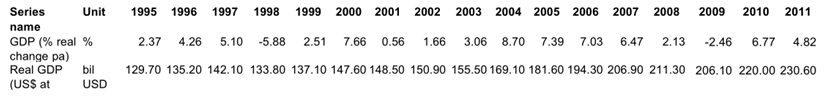
\includegraphics[width=1\textwidth]{hk1.png}
\caption{Data}
\label{threadsVsSync}
\end{figure}
%\begin{table}[htbp]
%\centering  
%\begin{tabular}{ccccccccccccccccccc} 
%\hline
%&Series  %name&Unit&1995&1996&1997&1998&1999&2000&2001&2002&2003
 %&2004&2005&2006&2007&2008&2009&2010&2011\\ \hline  % \hline
% &GDP(\% real change pa)&\%&2.37&4.26&5.10&-5.88&2.51&7.06&0.56&1.66&3.06&8.70&
% &7.39&7.03&6.47&2.13&-2.46&6.77&4.82\\    
% \hline
%\end{tabular}
%\caption{Trade for the last victim: Gaizhen %Wang}
%\end{table}
\end{frame}

\begin{frame}
\frametitle{The Influence of Economic Crisis on Hong Kong }
The real GDP from 1995 to 2011.
\bigskip
\begin{figure}[h]
\raggedleft
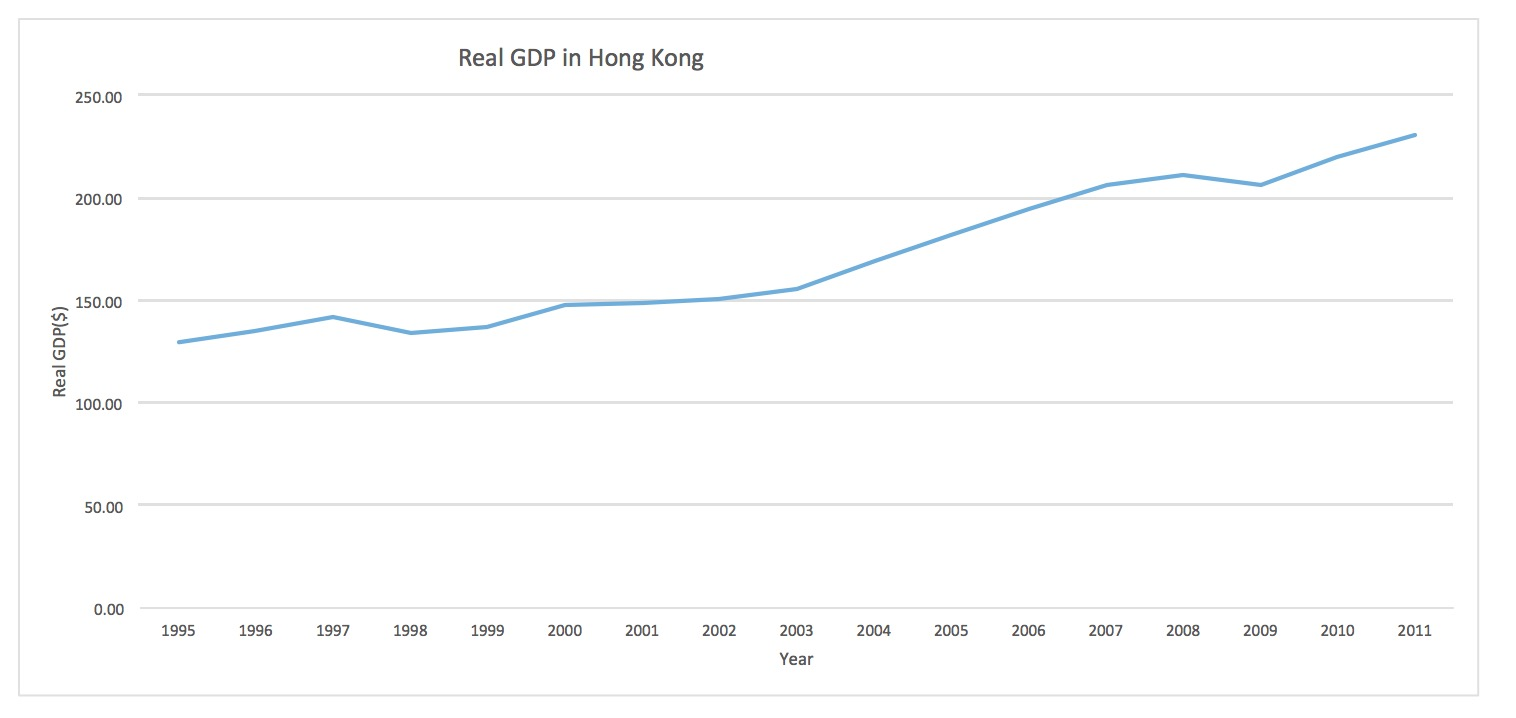
\includegraphics[width=1\textwidth]{hk2.jpg}
\caption{The real GDP}
\label{threadsVsSync}
\end{figure}
\end{frame}

\begin{frame}{The Influence of Economic Crisis on Hong Kong }
GDP growth rate from 1995 to 2011 in Hong Kong.\\
\bigskip
\begin{figure}[h]
\raggedleft
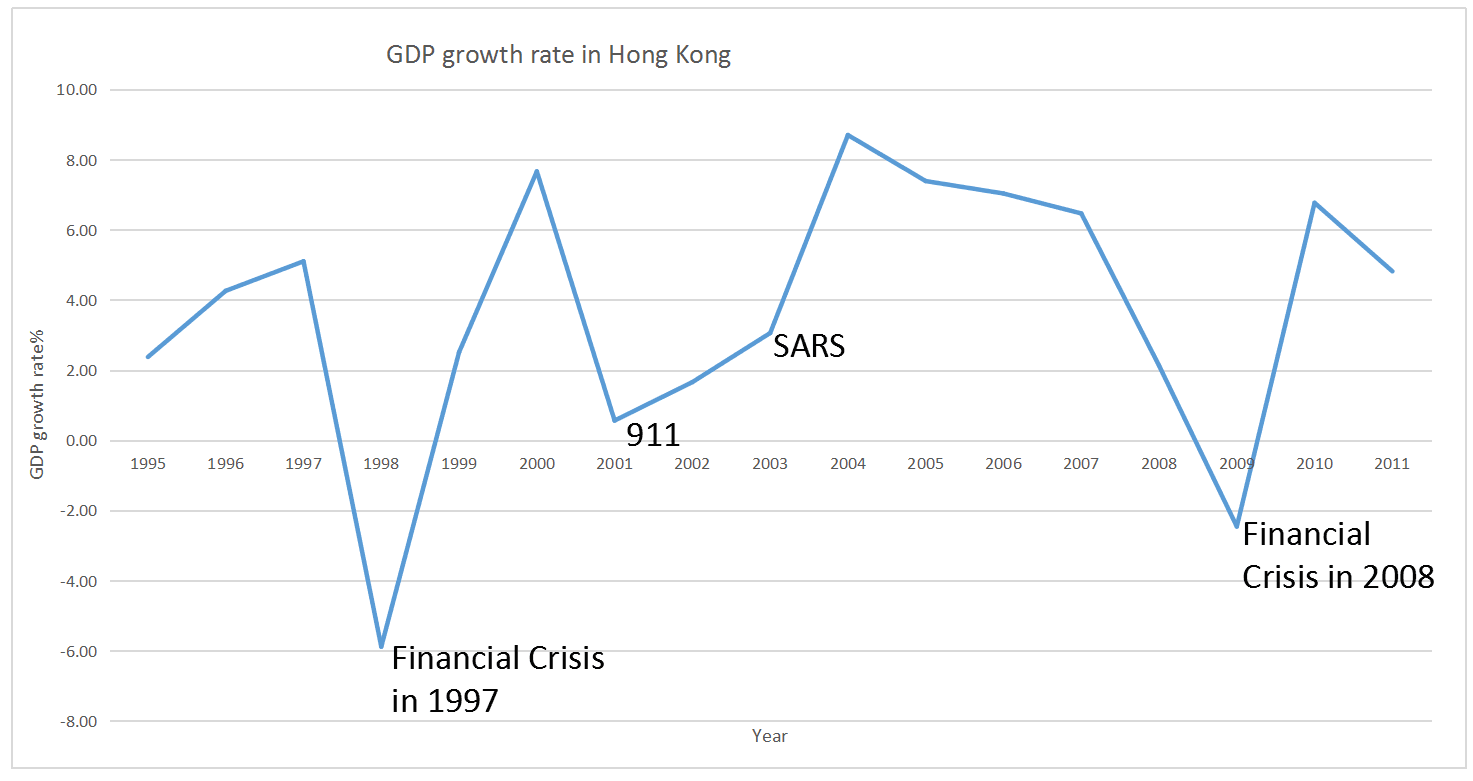
\includegraphics[width=0.9\textwidth]{hk23.png}
\caption{GDP growth rate}
\label{threadsVsSync}
\end{figure}
\end{frame}

\subsection{Explanation}
\begin{frame}{The Influence of Economic Crisis on Hong Kong }
Explanation\\
\bigskip
\alert{Financial Crisis in 1997}
\bigskip

\begin{enumerate}[i]
\pause\item International speculators have two “attacks” in Hong Kong.
\bigskip
\pause\item Use USD to change for Hong Kong dollar, increase exchange rate, change back.
\bigskip
\pause\item A panic in Financial market and less investment, less GDP.
\end{enumerate}

\end{frame}

\begin{frame}
\frametitle{The Influence of Economic Crisis on Hong Kong }
Explanation\\
\bigskip
\alert{Financial Crisis in 1997}
\bigskip
\begin{enumerate}[I]
\item <+-| alert@+> The poor credit borrow money to buy houses.

\bigskip
\item <+-| alert@+> Price of houses falls. Unable to pay back.

\bigskip
\item <+-| alert@+> Banks are less willing to lend. World economy came into recession.


\bigskip

\end{enumerate}
\end{frame}
\subsection{Huang}
\begin{frame}
\title {The Rise of China's Economy on Hong Kong's Economic Status}
\date{}
\titlepage
\end{frame}
\begin{frame}{The rise of China's Economy}
Structure\\
\begin{itemize}
\item Hong Kong's special economic status for China\\
\item The rise of China's economy\\
\item The impact on Hong Kong's economic status\\

\end{itemize}

\end{frame}
\begin{frame}
\frametitle{The rise of China's Economy}
The Special Economic Status of Hong Kong\\
\bigskip
\animate<1-3>%
\begin{itemize}[<+->]
\item The leading economic zone: “ Dragon's Head ”.
\item The mediation role on investment, capital introduction and the processing trade.
\item The financial center: provide offshore financial services.
\end{itemize}
\pause
\end{frame}





\subsection{close relationship}
\begin{frame}{The rise of China's Economy}
The Close Economic Relationship\\
\bigskip
\begin{overprint}
\onslide<1>
The economic return runs before the political return.\\
\begin{figure}[h!]
\centering
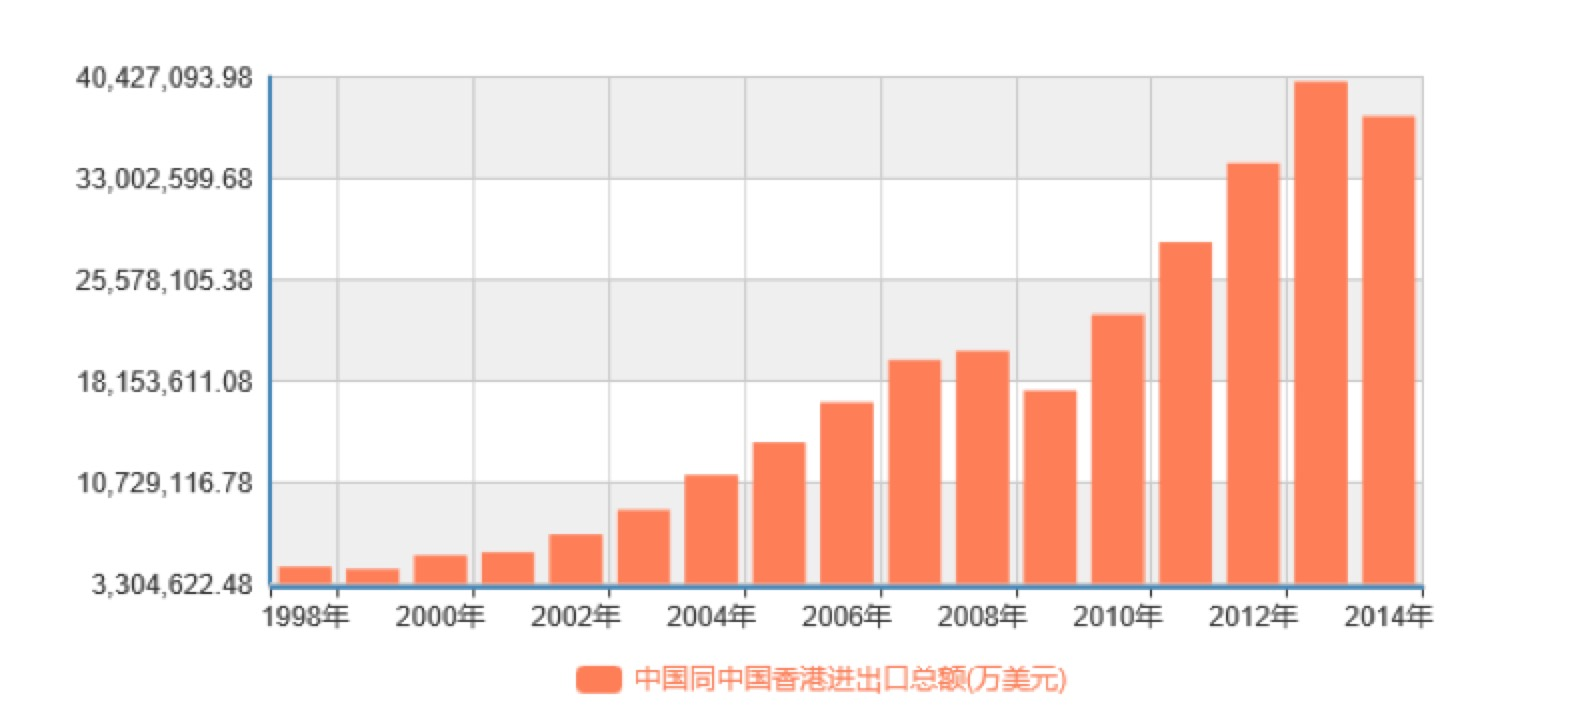
\includegraphics[width=0.9\textwidth]{hk6.jpg}
\label{threadsVsSync}
\end{figure}
\onslide<2>
Case: In 1980s,  the north movement of manufacture industries contributed to the economic development of Guangdong.\\ 
\begin{figure}[h!]
\centering
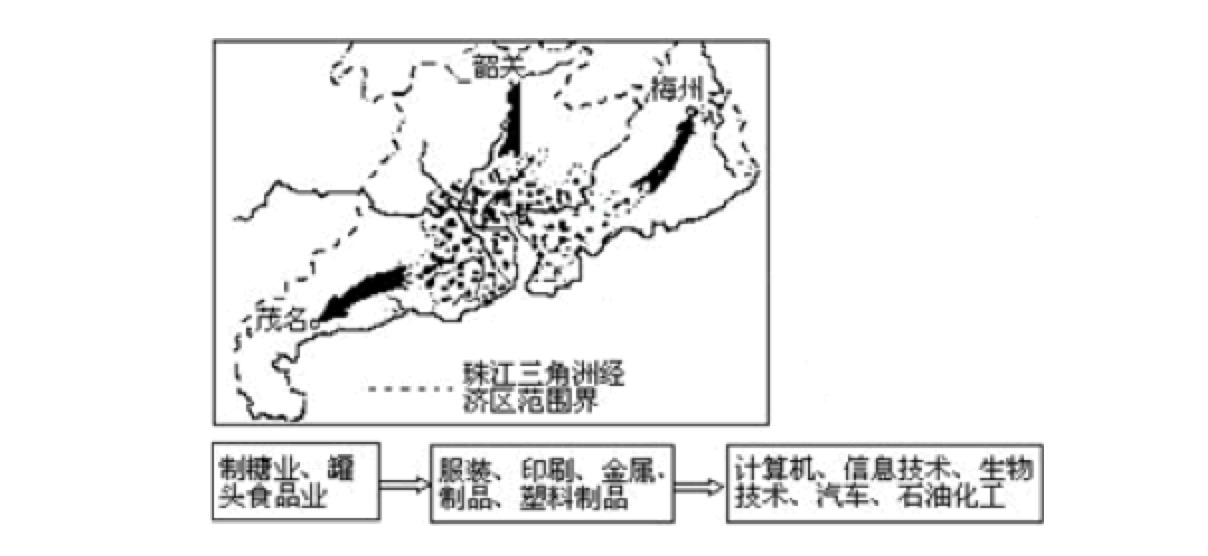
\includegraphics[width=0.7\textwidth]{hk7.jpg}
\label{threadsVsSync}
\end{figure}
\end{overprint}
\end{frame}


\subsection{Rise}
\begin{frame}
\frametitle{The rise of China's Economy}
The rise of China's Economy\\
An economic miracle.\\
\bigskip
\begin{figure}[h!]
\centering
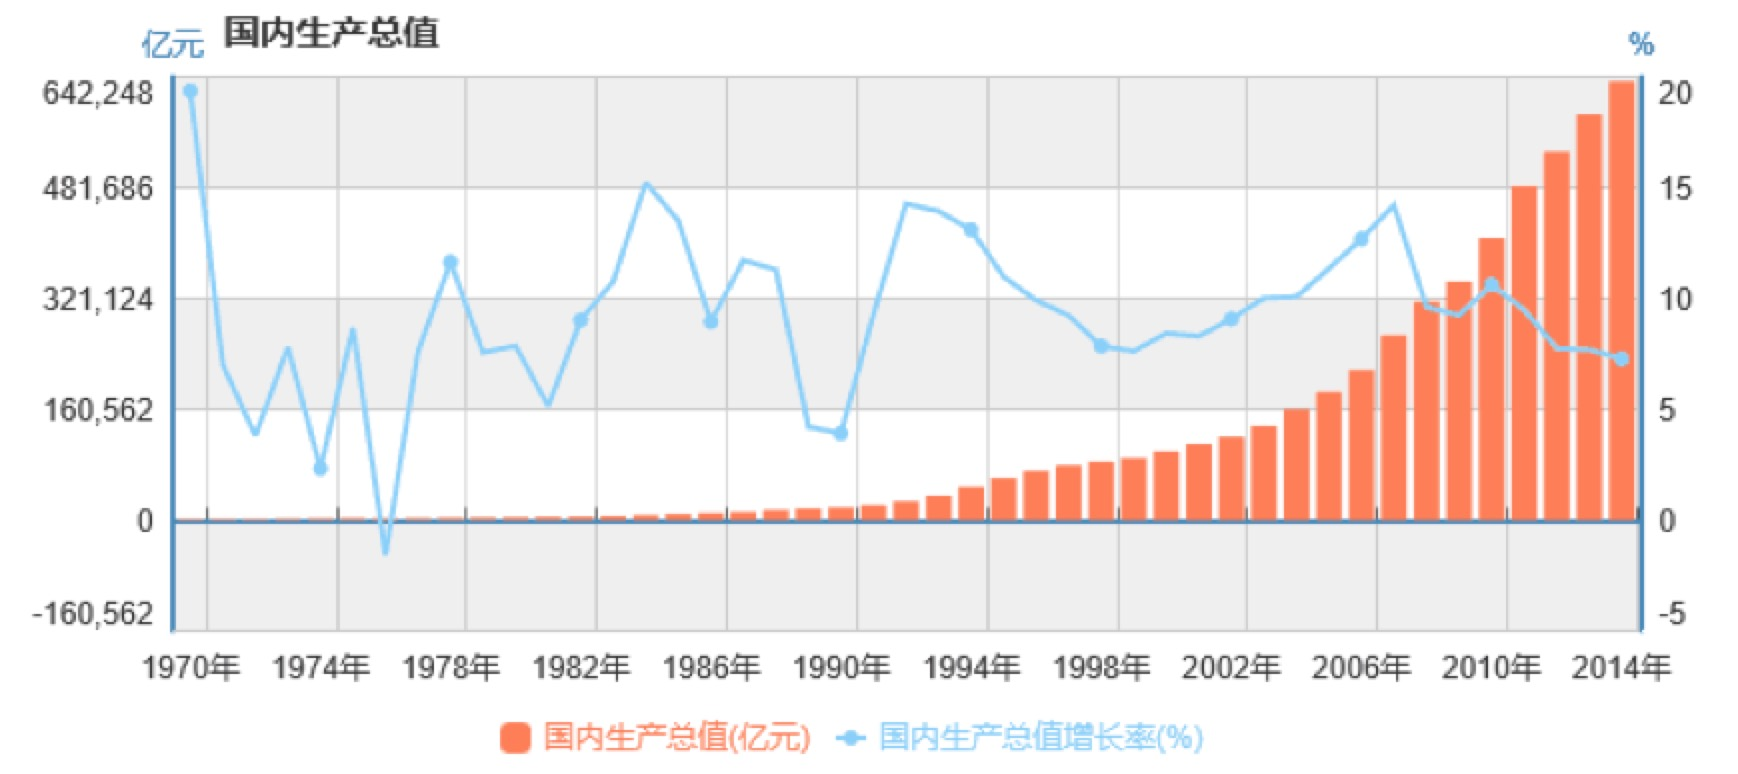
\includegraphics[width=1\textwidth]{hk8.jpg}
\label{threadsVsSync}
\end{figure}
\end{frame}


\begin{frame}{The rise of China's Economy}
The impact on Hong Kong's economic status\\
\bigskip
From the perspective of the background of Hong Kong's rise\\
\bigskip
\bigskip
Shanghai financial center went to the weak
$\Longrightarrow$ the rise of Shanghai, Beijing and Shenzhen\\
\bigskip
\bigskip
The economic autarky situation, the planned economy
$\Longrightarrow$ The more open economy, the maket economy.\\
\bigskip
\bigskip
The lack of bridge between China and foreign countries
$\Longrightarrow$ The second largest international trade country.\\
 



\end{frame}
\begin{frame}
\bigskip
\bigskip
\bigskip
\bigskip
\bigskip
\bigskip
\bigskip
\bigskip
Shanghai financial center went to the weak
$\Longrightarrow$ the rise of Shanghai, Beijing and Shenzhen\\
\bigskip
\bigskip
\end{frame}


\begin{frame}
\frametitle{The rise of China's Economy}

\begin{figure}[h!]
\centering
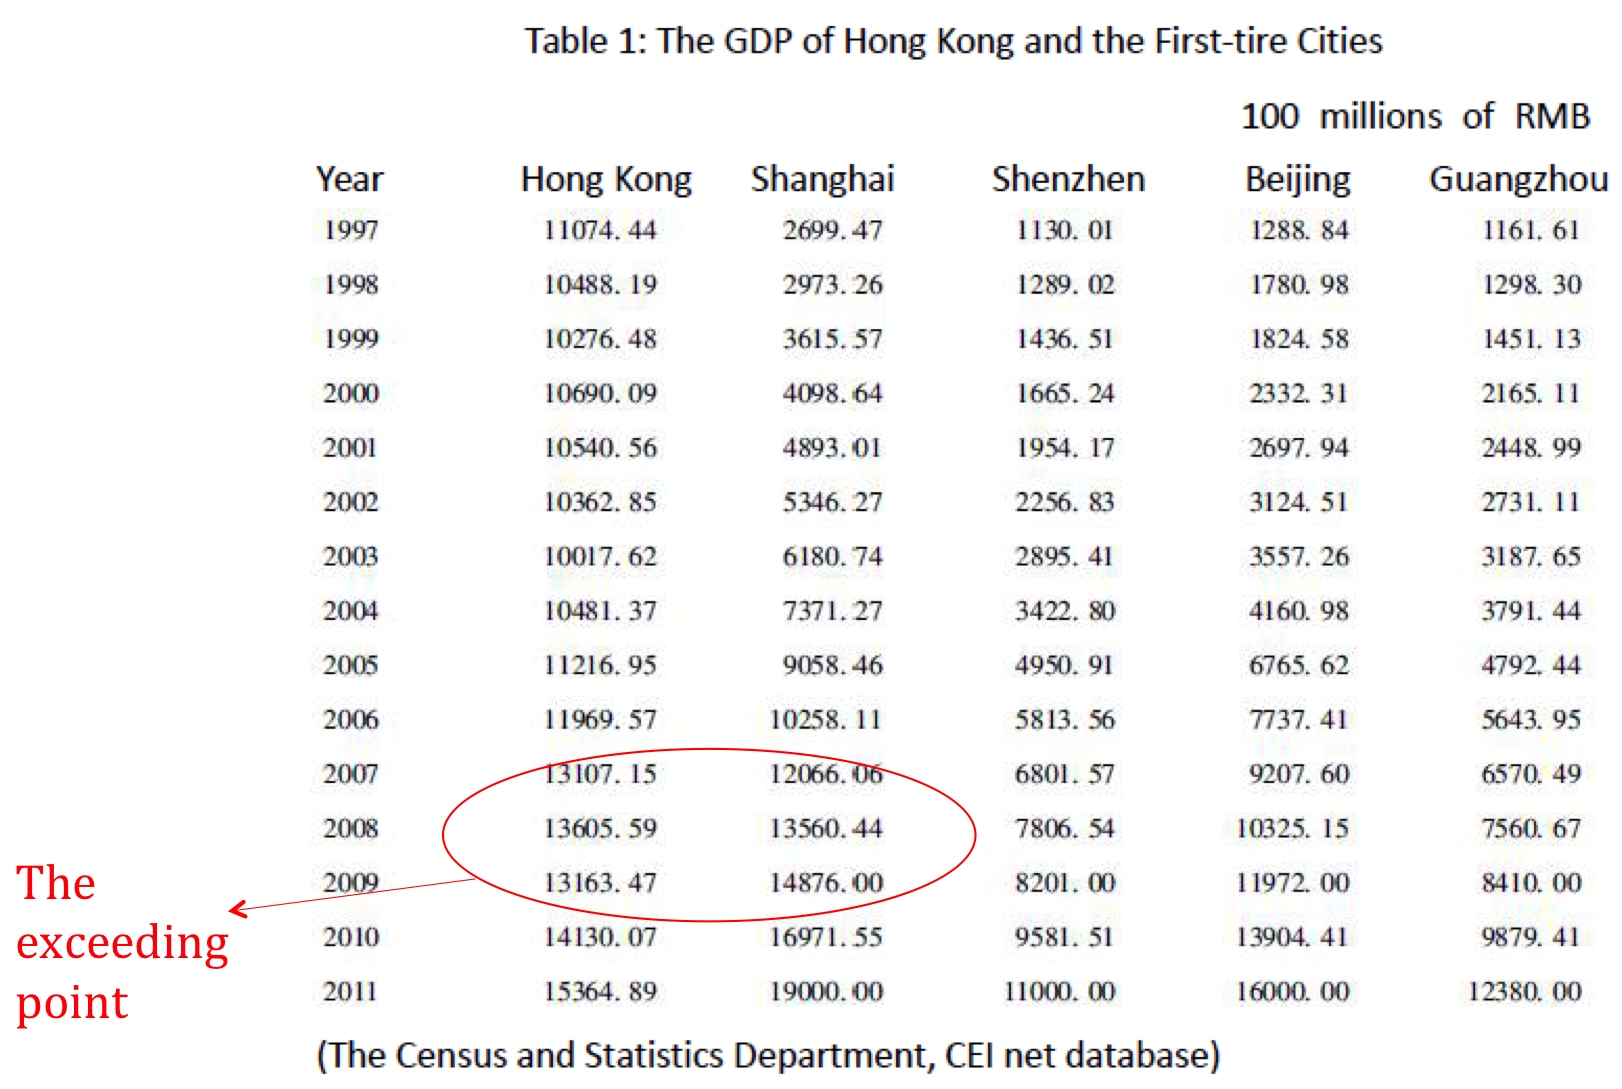
\includegraphics[width=0.9\textwidth]{hk8.png}
\label{threadsVsSync}
\end{figure}
\end{frame}

\begin{frame}{The rise of China's Economy}
The economic autarky situation, the planned economy
$\Longrightarrow$ The more open economy, the maket economy.\\
\begin{figure}[h!]
\centering
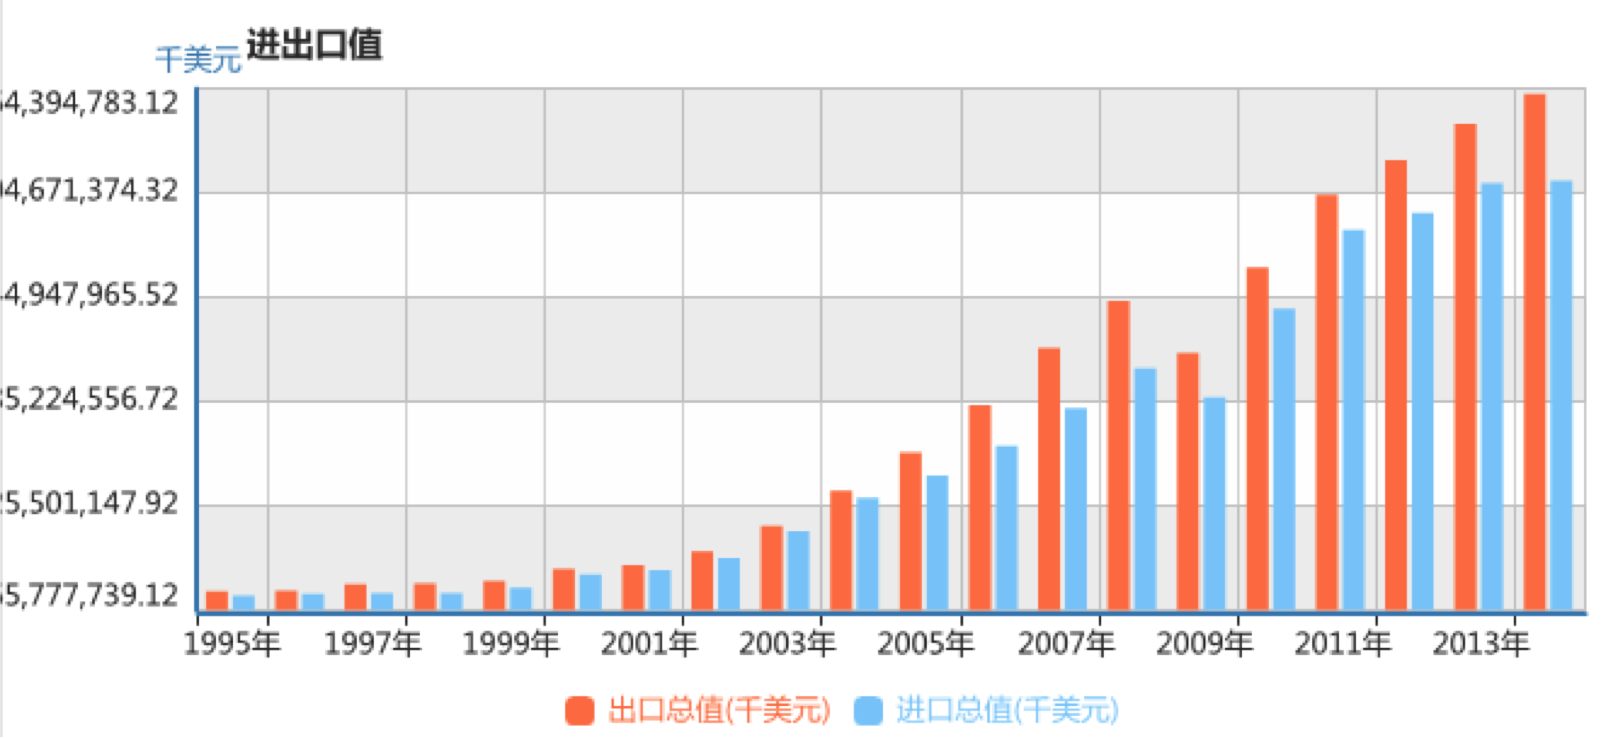
\includegraphics[width=0.9\textwidth]{hk24.png}
\label{threadsVsSync}
\end{figure}

\end{frame}
\subsection{High Density}
\begin{frame}
\frametitle{The rise of China's Economy}
The high economic density $\Longrightarrow$ the fast development of China.
\\
\bigskip
\center{In 1978}
\begin{figure}[h]
\centering
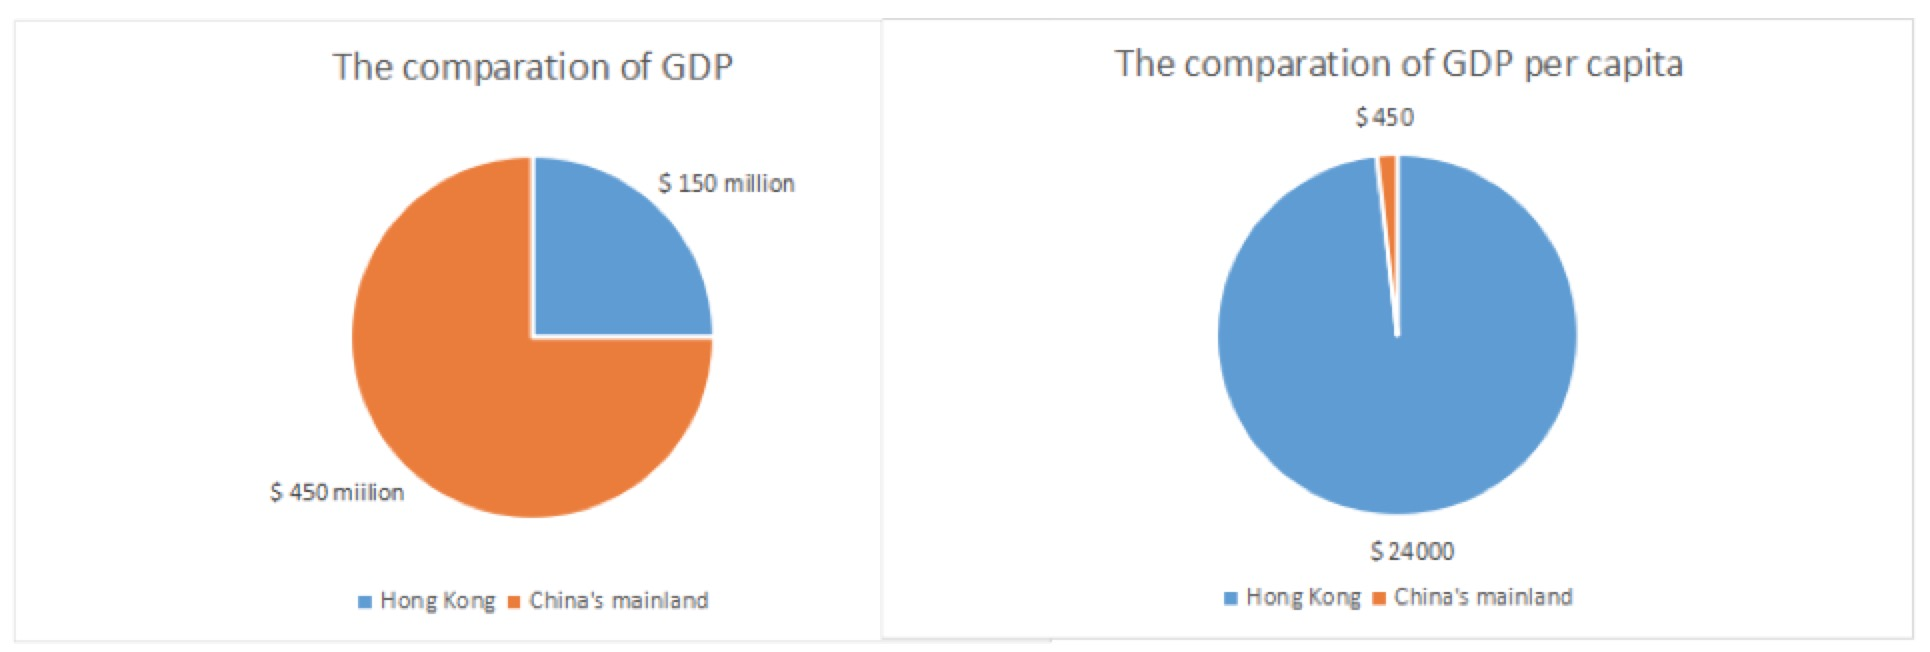
\includegraphics[width=1\textwidth]{hk5.jpg}
\label{threadsVsSync}
\end{figure}
~~~~~~~~~~~~~~~~~~~~~~~~~~~~~~~~~~~~~~~~~~~~~~~~Shanghai \$$3000$
\end{frame}
\begin{frame}
\frametitle{The rise of China's Economy}
\begin{figure}[h]
\centering
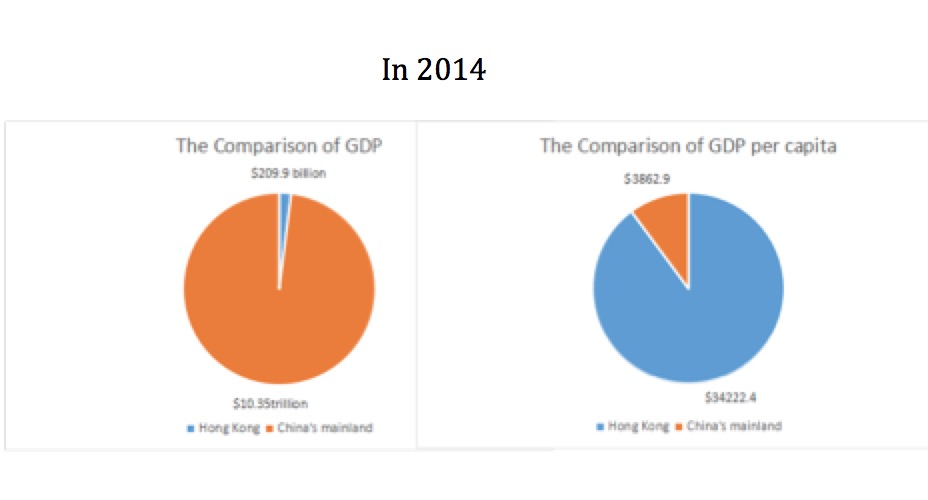
\includegraphics[width=1\textwidth]{hk25.png}
\label{threadsVsSync}
\end{figure}
\end{frame}

\subsection{The impact on Hong Kong's economic status}
\begin{frame}
\frametitle{The rise of China's Economy}
\textcolor{red}{The impact on Hong Kong's economic status}\\
\bigskip
From the perspective of the institutinal reasons\\

\bigskip
\begin{itemize}
\item Government's policy change.
\bigskip
\item Political institutional contradiction.
\bigskip
\item Different economy system on tax, trade, accounting policy.
\end{itemize}

\end{frame}

\begin{frame}{The rise of China's Economy}

\transwipe<1>
\textcolor{red}{The impact on Hong Kong's economic status}\\
\bigskip
From the perspective of the cultural reasons.\\
\bigskip
\begin{itemize}
\item The rise of Hong Kong’s native consciousness.
\bigskip
\item The miss of British ruling.
\end{itemize}


\end{frame}

\section{Conclusion}
\subsection{con}
\begin{frame}{Conclusion}

\bigskip
\bigskip

\begin{block}{\center{Conclusion}}
Now, we can draw the conclusion that the reasons which lead to the fall of Hong Kong's economy are internal cause: \alert{the economic competitiveness of Hong Kong}  
and the external causes: \alert{the return of Hong Kong, the economic crisis and the rise of mainland China}.
\end{block}
\end{frame}
\begin{frame}
\transsplitverticalin<1>
\bigskip
\bigskip
\bigskip
\bigskip
\bigskip
\bigskip
\bigskip


\center{Thank}\\ 
\center{YOU}
\end{frame}
\end{document}
